%!TEX encoding = UTF-8 Unicode
%%%%%%%%%%%%%%%%%%%%%%% file template.tex %%%
%%%%%%%%%%%%%%%%%%%%%%
%
% This is a general template file for the LaTeX package SVJour3
% for Springer journals.          Springer Heidelberg 2010/09/16
%
% Copy it to a new file with a new name and use it as the basis
% for your article. Delete % signs as needed.
%
% This template includehttps://www.overleaf.com/18909956dygyghmktbjfs a few options for different layouts and
% content for various journals. Please consult a previous issue of
% your journal as needed.
%
%%%%%%%%%%%%%%%%%%%%%%%%%%%%%%%%%%%%%%%%%%%%%%%%%%%%%%%%%%%%%%%%%%%
%
% First comes an example EPS file -- just ignore it and
% proceed on the \documentclass line
% your LaTeX will extract the file if required
\begin{filecontents*}{example.eps}
%!PS-Adobe-3.0 EPSF-3.0
%%BoundingBox: 19 19 221 221https://www.overleaf.com/18909956dygyghmktbjf
%%CreationDate: Mon Sep 29 1997
%%Creator: programmed by hand (JK)
%%EndComments
gsave
newpath
  20 20 moveto
  20 220 lineto
  220 220 lineto
  220 20 lineto
closepath
2 setlinewidth
gsave
  .4 setgray fill
grestore
stroke
grestore
\end{filecontents*}
%
\RequirePackage{fix-cm}
%
%%\documentclass{svjour3}                     % onecolumn (standard format)
%%\documentclass[smallcondensed]{svjour3}     % onecolumn (ditto)
\documentclass[smallextended]{svjour3}       % onecolumn (second format)
%\documentclass[twocolumn]{svjour3}          % twocolumn
%
\smartqed  % flush right qed marks, e.g. at end of proof
%
\usepackage{amsmath,amsfonts,amssymb}
\usepackage[latin1]{inputenc}
\usepackage{graphics} %%
\usepackage{graphicx}
\usepackage{subfigure} 
\usepackage[colorlinks=true, allcolors=blue]{hyperref} 
\usepackage[ngerman,english]{babel} 
\usepackage{lineno}
\usepackage{lscape} 
\usepackage{rotating} 
%%\usepackage{natbib} 
\usepackage{color}
\usepackage{soul}
\usepackage{xcolor,colortbl}
% etc.
%
% please place your own definitions here and don't use \def but
% \newcommand{}{}

\newcommand{\tem}[1]{\textcolor{red}{Teresa Mineo: #1}} %Teresa's comments
\newcommand{\anto}[1]{\textcolor{green}{Antonello: #1}} %
\newcommand{\rob}{\textcolor{orange}} 

%\newcommand{\xmm}{\textit{XMM-Newton}}
%\newcommand{\erosita}{\textit{eROSITA}}
%\newcommand{\athena}{\textit{ATHENA}}
\linenumbers
\usepackage{marvosym}

%
% Insert the name of "your journal" with
% \journalname{myjournal}
%
%%\journal{}

%------------------------------------------------------------------------------
% Code for ORCID iD
%------------------------------------------------------------------------------
\usepackage{tikz,xcolor,hyperref}

% Make Orcid icon
\definecolor{lime}{HTML}{A6CE39}
\DeclareRobustCommand{\orcidicon}{%
	\begin{tikzpicture}
	\draw[lime, fill=lime] (0,0) 
	circle [radius=0.16] 
	node[white] {{\fontfamily{qag}\selectfont \tiny ID}};
	\draw[white, fill=white] (-0.0625,0.095) 
	circle [radius=0.007];
	\end{tikzpicture}
	\hspace{-2mm}
}

\foreach \x in {A, ..., Z}{%
	\expandafter\xdef\csname orcid\x\endcsname{\noexpand\href{https://orcid.org/\csname orcidauthor\x\endcsname}{\noexpand\orcidicon}}
}

% Define the ORCID iD command for each author separately.
\newcommand{\orcidauthorA}{0000-0003-4727-9136}
\newcommand{\orcidauthorB}{0000-0002-4931-8445}
\newcommand{\orcidauthorC}{0000-0001-8722-0361}
\newcommand{\orcidauthorD}{0000-0002-9554-4128}
\newcommand{\orcidauthorE}{0000-0001-9204-9749}

\begin{document}

%\title{A semi-empirical model for soft proton scattering at grazing incidence from X-ray mirrors}
\title{The ASTRI-Horn telescope: evaluation of the diffuse night sky background and comparison with UVscope measurements}

%\thanks{Grants or other notes
%about the article that should go on the front page should be
%placed here. General acknowledgments should be placed at the end of the article.}

%\subtitle{Do you have a subtitle?\\ If so, write it here}

\titlerunning{ASTRI-Horn Bkg}        % if too long for running head

\author{Antonio~Alessio~Compagnino\textsuperscript{\Email}\orcidA{} \and Teresa~Mineo\orcidB{} \and Maria~Concetta~Maccarone\orcidC{} \and Osvaldo~Catalano\orcidD{} \and Domenico~Impiombato\orcidE{}}


%\authorrunning{Short form of author list} % if too long for running head
\authorrunning{A.~Compagnino, T.~Mineo, M.C.~Maccarone, O.~Catalano, D.~Impiombato}
\institute{Alessio~Compagnino \and Teresa~Mineo \and Maria~Concetta~Maccarone \and Osvaldo~Catalano \and Domenico~Impiombato\at
              INAF, Istituto di Astrofisica Spaziale e Fisica Cosmica di Palermo, via U. La Malfa 153, I-90146 Palermo, Italy \\ 
              \Email\texttt{\scriptsize{ :alessio.compagnino@inaf.it}}         
           }

\date{Received: date / Accepted: date}
% The correct dates will be entered by the editor

\maketitle

\begin{abstract}
.....


\keywords{}
% \PACS{PACS code1 \and PACS code2 \and more}
% \subclass{MSC code1 \and MSC code2 \and more}
\end{abstract}

\section{Introduction}
\label{sect:intro}


%\textit{\textcolor{blue}{\hl{Cettina: primo draft }}}

\begin{itemize}
\item
ASTRI-Horn (Cettina)
\item
UVscope (Cettina)
\item
task of the article 
\end{itemize}
\section{ASTRI-Horn telescope} 
The ASTRI-Horn telescope is based on a dual mirror system in Schawrzschild-Couder configuration
with a focal length of 2.15 m and a nominal field of view (FoV) of 9.6$^\circ$. 
The primary mirror, 4.3 m diameter, is segmented in 18 hexagonal panels, 
while the secondary mirror, 2.2 m diameter, is a monolitic hemispherical thick glass shell. 
Dedicated measurements  with an optical CCD camera showed that the
point spread function (PSF) has a constant width of a few arcmin
over the whole FoV and that  90\% of the PSF  is containerd in one camera pixel (ref)
whose angular size is 0.19$^\circ$. 
However, in the observation analysed, three of panels were not in their proper condition:
one of them was covered because not adjustable through the active mirror control, the other two were found to be misaligned by $\sim$1$^\circ$ by means of a dedicated analysis based on the variance method.
In addition, the secondary mirror experienced a degradation of the reflectivity because of a strong eruption of the Etna volcano on February 2019, and all the following observations were affected by loss of about 25\% of the optical throughput
respect to the December one \cite{Mineo2019}. 

The focal surface camera, has a convex-shaped structure where
photon detection modules (PDMs), that are square flat modules, are symmetrically placed
with angles respect to the telescope axis opportunely chosen in order to follow the curvature of the focal plane.
Currently, the camera includes 21 out of 37 PDMs, for a total effective FoV of 7.6$^\circ$.
A skeme of the disposition of the PDM is presented in Fig.~\ref{fig:camera}, where numbers identifying each PDM are also indicated. 
\begin{figure}
%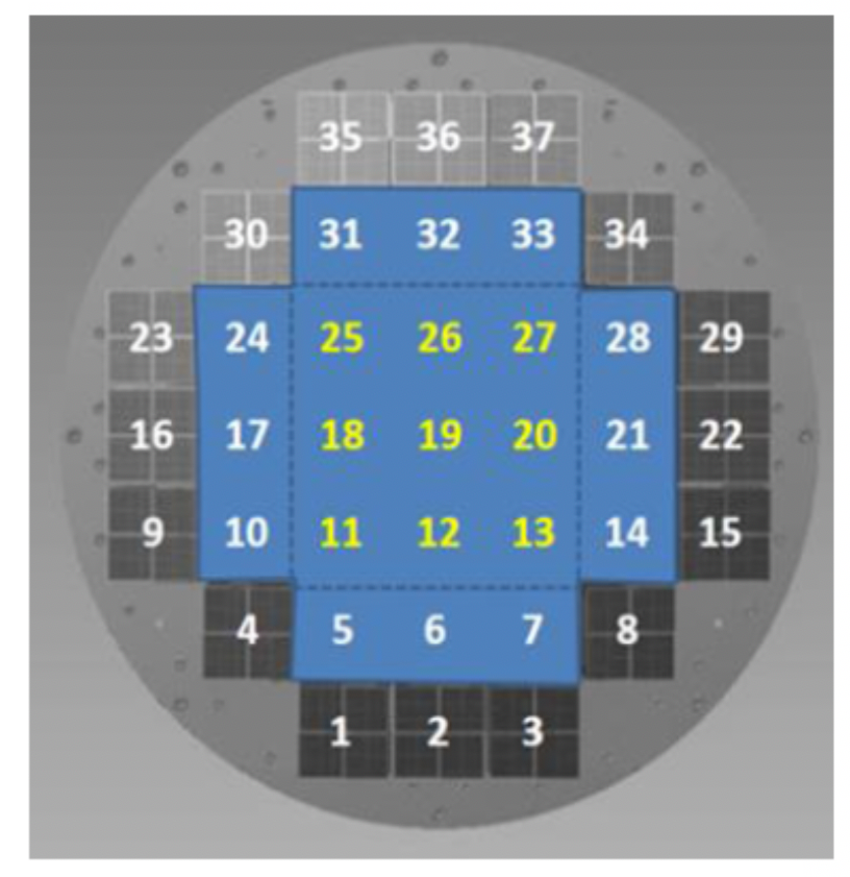
\includegraphics[height=7.9cm,angle=0,scale=1.0]{focal_plane.ps}
\caption{Skeme of the disposition of the PDMs on the focal surface. Numbers identify the PDM, the FoV common to UvScope is indicated with the dashed lines and with the yellow color of the PDMs.}
\label{fig:camera}
\end{figure}

Each PDM, composed of 8$\times$8 side-by-side Silicon photomultipliers (SiPMs), 
is installed on a printed circuit board that hosts the front-end electronics (FEE) composed by
 two application specific integrated circuits (ASIC) for the SiPM signal read out.
 The ASTRI camera FEE electronics \cite{Sottile2016} represents an innovative solution, being based on a custom peak-detector operation mode to acquire the SiPM pulses rather than the sampling technique usually adopted by other Cherenkov telescopes.
This FEE-FPGA manages the the generation of local trigger, a topological one, activated when a given number of contiguous pixels within a PDM presents a signal above a given photo-electron threshold \cite{Sottile2016}.
The back-end electronics (BEE) is the main elaboration unit of the camera which
controls and manages the overall system, including data, and
all ancillaries used to perform operations as
the camera thermal regulation, the voltage distribution management and the time events stamping.
The BEE also provides the functions necessary to process and transmit the event data as 
obtained by the FEE to an external data acquisition 
workstation responsible for receiving and storing the data packets \cite{Sottile2016}.
In order to protect the camera sensors from the external
atmospheric environment, an optical-UV transparent poly methyl methacrylate (PMMA)  window 
is mounted onto the focal surface support structure covering all the PDMs.
This window is modeled with the same radius of curvature of the focal surface \cite{Catalano2018}.
The ASTRI SST-2M camera is also equipped  with a light-tight lid to prevents accidental sunlight 
exposure of the focal surface detectors.
The camera is thermally controlled to keep the working temperature on the focal plane within the range 13-17$^\circ$C
for maintaing a goopd gain stability.


ASTRI-Horn read out electronics is AC-coupled to the detector output, and any slow varying signal is  blocked.
The camera is then blind to the diffuse night sky background (NSB) or to the light from stars in the FoV.   However, considering that sky photons actually arrive with a random Poissonian time distribution, the fluctuations generated in the electronic signal are detected as noise. ASTRI-Horn  background is then caracterised by signals distributed around an constant average value (pedestal) with fluctuations whose standard deviation is due both to the intrinsic electronic noise and to the NSB flux.  The total standard deviation of the background in the camera is obtained by the following formula:

\begin{equation}
\sigma^2=\sigma^2_{dk}+\sigma^2_{sky}
\end{equation}

\noindent
where $\sigma_{dk}$ is the intrinsic standar deviation of the electronics plus the detector noise observed in complete dark condition, as with the lid closed, and $\sigma_{sky}$ is the standard deviation induced by the  NSB  which is directly proportional to the photon flux.


\section{ASTRI-Horn data reduction and analysis} 
\label{sect:astridata}

\subsection{Gain evaluation}
\label{subs:gain}

A first step of the data analysis chain is the gain calibration of the camera pixels. 
ASTRI-Horn camera is equipped with a thermal control system to monitor the temperature of the focal plane and coherently change the voltage applied to the SiPM in order to keep gain variation within a few ADC. In addition, a dedicated procedure is forseen to evaluate off-line the gain in each observing period with the accuracy required for the scientific analysis ({\tem mettere il valore} ADC). This method is based on the use of a side emitting fiber optics system (FOC) located along the PMMA window circumference and connected to a controlled intensity diode (LED) lightning  almost uniformly  the focal plane with an average intensity of a few $p.e.$ per pixel. FOC data are collected periodically during the normal telescope acquisition mode (???).

FOC data used for this paper data analyis are listed in Table~\ref{tab:FOC}; they are relative to a fixed voltage $V_{0}$= 57 V {\tem di che?} and a temperature of 15$^\circ$C {\che vuol dire?}. For these acquisitions HG data are available.

The pulse hight distribution for each considered run is accumulated and the  maximum amplitude 
for all the recorded waveforms of a physical pixel. While the first peak is the pedestal, the following  ones are the single and multiple p.e. contributions. The distance between 
the peaks allow to extract the conversion factor.

Figure~\ref{fig:FOC} shows the HG pulse height spectrum acquired in the FOC run \tem{quale?}. 


\begin{figure*}[ht!!]
\centering
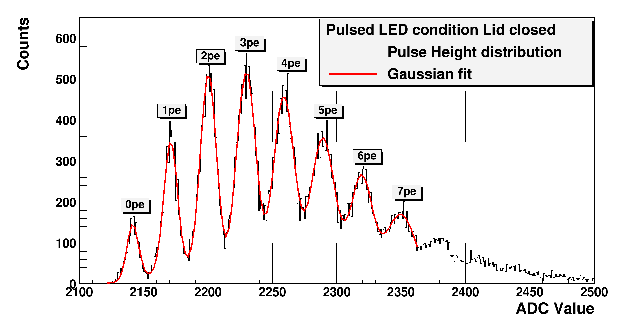
\includegraphics[angle=0, width=12.5cm]{PIXEL60_PDM20_HG_DICEMBRE_2018.eps}
\vspace{0.5cm}
\caption{ Pulse height spectrum at a fixed temperature of 15$^\circ$C
and $V_{0}$=57 V for a camera pixel, during a FOC run in the HG electronics chain. 
The black curve represents the distribution of the peak detector output and the red curve shows the corresponding
multiple peaks Gaussian fit.}
\label{fig:FOC}
\end{figure*}

\begin{table*}[htbp!!]
\centering
\caption{Log of FOC data used in the analysis. For these runs HG data are considered. }
\label{tab:FOC}
\begin{tabular}{lccc}
\hline\hline
Obs. ID & Starting Date &  Expopsure & Number of events \\
               & (year/month/day h:m:s) & (s)   \\
\hline     
1394 & 2018/12/02 20:01:09  &  & 60065     \\
1763 & 2019/03/23 20:01:21  &  & 120123    \\ 
\hline\hline
\end{tabular}
\end{table*}

\subsection{Open sky data} 
\label{subs:skydata}

Background data used for the analysis refer to the period between December 2018 and March 2019 when the telescope was mainly involved in the Crab observation campaign. The list of the considered run ID is reported in Table~\ref{tab:obslog}; runs are split in several files, each containing a maximum of 50000 events, identified with a progressive number.
A selection was applied in order to avoid data affected by technical problems as instability in the PDM signals or fluctuation of the trigger rate. Moreover, intervals with bad atmospheric conditions 
(high humidity, low external temperature, cloudiness) were not considered as well as the periods when UVscope data are not available.

In each detected events we considered only the nine central PDM (11, 12, 13, 18, 19, 20, 25, 26, 27 in Fig.~\ref{fig: camera} ) taking into account the smaller UVscope FOV.  In addition, bad pixels and pixels imaging stars with a magnitude higher than …, coherently with the procedure adopted for UVscope data, are excluded from the analysis. The position of the stars in ASTRI-Horn FOV is computed from the correspondence with UVscope pixels derived from the variance method (Segreto et al 2019). 
The variance method was not used to identify stars because the relative data were not available in December and, for uniformity in the analysis, we decide to not use it either in March.  However, March variance data were used to cross-check the positions obtained from the correspondence with UVscope pixels.


\begin{table}[ht]
\label{tab:astrilog}
\caption{ASTRI-Horn observation log}
\centering
\begin{tabular}{lcccc}
\hline\hline
Observation ID & Starting Date & Exposure      & Number of events & pointing \\
               & (year/month/day h:m:s) & (s)  \\
\hline     
%https://www.overleaf.com/project/5e3005eb54e0d8000155a7ff

1429 & 2018/12/05 20:57:37  &   2094     & 31755 & Crab Off    \\
1430 & 2018/12/05 21:54:40  &   909      & 29808 & Fixed AltAzi Azi$=180°$ EleV. $=70°$    \\
1453 & 2018/12/07 20:06:11  &   6016     & 348442 & Crab Off    \\
1453 & 2018/12/07 20:06:11  &   6016     & 348442 & Crab Off    \\
1453 & 2018/12/07 20:06:11  &   6016     & 348442 & Crab Off    \\
1453 & 2018/12/07 20:06:11  &   6016     & 348442 & Crab Off    \\



1453 & 2018/12/07 20:06:11  &   6016     & 348442 & Crab Off    \\
1454 & 2018/12/07 22:09:16  &   4377     & 226651 &  Crab \\ %226650  \\
1455 & 2018/12/07 23:30:08  &   6243     & 412451 &  Crab \\ %412446    \\
1456 & 2018/12/08 01:24:48  &  8530     & 237318 & Crab Off \\ %  237186 \\
1457 & 2018/12/07 03:50:20  &  3509     & 126295 & Fixed ALtAzi\\ % 126264   \\
1464 & 2018/12/08 20:30:37 &  2255 & 97257 & Crab Off \\ %97251 \\  
1465 & 2018/12/08 21:17:34 &  9624 & 430245 & Crab\\ % 430222\\  
1466 & 2018/12/09 00:07:25 &  3161 & 251442 & Crab \\ %251418  
1467 & 2018/12/08 01:09:44 &  8959 & 243713 & Crab Off \\ %243399
1468 & 2018/12/08 03:40:11 &  1237 & 33168 &  Fixed AltAzi\\ %33126
1658 & 2019/03/05 18:13:58 &  112 & 1435 & Merak \\  
1659 & 2019/03/05 18:19:26 &  154 & 3149 & Zeta Tauri \\  
1660 & 2019/03/05 18:24:37 &  6224  & 419636 & Crab \\ %419631  
1661 & 2019/03/05 20:10:15 &  168 & 14389 & Zeta Tauri \\  
1662 & 2019/03/05 20:19:59 &  4008 & 198186 & Crab Off \\   
1663 & 2019/03/05 21:29:34 &  2337 & 165264 &  Fixed AltAzi \\  
1670 & 2019/03/06 18:08:27 &  628    &   8191      &  Merak\\
1671 & 2019/03/05 18:21:51 &  126        &   2412   & Zeta Tauri \\
1672 & 2019/03/05 18:25:56 &  5935    &   296073   &  Crab \\ %296046
1673 & 2019/03/05 20:06:58 &  183      &   3272     & Zeta Tauri\\ %3270
1674 & 2019/03/05 20:13:37 &  13812      &    152393 & Crab Off  \\ %152110     \\
%1466 & 2018/12/09 20:47:50 &  1218 & 50000 \\  

\hline\hline
\end{tabular}
\end{table}

Background pixels were identified applying the same double cut cleaning procedure used for the Cherenkov shower images. This procedure considers background pixels the ones that have a signal lower than a first threshold $S1$, or , if higher than $S1$, with none of the neighboring pixels with a signal higher that the second threshold $S2$. In our analysis, we adopted the values $S1$=6 and $S2$=12 used by Mineo et al. 2019 instead of higher values adopted for the analysis of Crab events (Lombarbi et al. 2018) to avoid muon signals.

For each event we then accumulated the distribution of the number of $p.e.$ in the background pixels. The curve obtained for the file 1473 of the run ID 000 is plotted in Fig.~\ref{fig:distr} as example. It is a distribution with a Gaussian shape in the central part and with long wings due to residual signals in the positive part and to … ???? in the negative one. 

The central part of the distribution is then fitted with a Gaussian whose $\sigma$ is the measure of the NSB fluctuations that, being a Poissonian signal, is linked to the absolute flux. The RMS values for December 9—10 observation night are plotted in Fig.~\ref{fig:rms} as function of time.

Finally, we plot the resulting values of $\sigma$ for each observing night in Fig.\ref{fig:sigma}  as a function of time. 


\subsection{Closed camera data} 




Dark counts runs are acquired when the lids of the camera are closed.
The light-tight lid, in addition to protecting the FSC, it ensures that no light can enter it when the lid is latched shut. In this way, it is possible to read out the pulse height of all the signals pixel for each triggered dark event.
In absence of light, using the Low Gain electronics chain, the majority of events are  contained in one peak position, named pedestal. 
It, that does not vary with temperature(\cite{Impiombato2016}), is considered as offset electronics chain in the analysis of cherenkov images for the astronomical observations.
Each pulse height spectrum of the camera pixels, is fitted with a Gaussian function, allowing to obtain the exact peak position value in the ADC counts with the relative width (see Fig.~\ref{fig2}).


\begin{table*}[htbp!!]
\centering
\caption{ASTRI-Horn FOC/Dark runs}
\label{table2}
\begin{tabular}{lccc}
\hline\hline
Run ID & Starting Date & Run type      & Number of events \\
               & (year/month/day h:m:s)   \\
\hline     
1380 & 2018/12/01 20:59:18  &   Dark    & 15305      \\
1394 & 2018/12/02 20:01:09  &   FOC     & 60065     \\
1616 & 2019/02/28 12:37:02  &   Dark    & 50000     \\
1763 & 2019/03/23 20:01:21  &   FOC     & 120123    \\
  

\hline\hline
\end{tabular}
\end{table*}

\newpage
\section{UVscope data reduction and analysis} (Cettina)
\label{sect:uvscopedata}

The data acquired by UVscope are registered, pixel by pixel, as number of counts in a pre-selected integration time; in our case we have set a rate of one acquisition each second. The conversion from counts to physical units is related to several features (geometrical factor, dark counts, average efficiency, gain uniformity) that characterize the sensor and its configuration, as widely detailed in \citep{Maccarone2020} and briefly reported in the following.  The geometrical factor, depending on the effective pixel area, pupil area and distance between pupil and photocathode, whose values have been indicated in a previous paragraph, corresponds to about 1.225~mm$^2{\times}$deg$^2$. The dark counts depend from the temperature but in our case, being UVscope thermally stabilized by the Peltier system, such noise has negligible values( 0.7~counts/second per pixel). The mean value of the global average efficiency of the sensor (comprehensive of collecting, trigger and quantum efficiencies) was obtained by NIST-calibration in lab (11.85\%) and adjusted for the quartz window, 99\% UV transparent , present in UVscope mounted aboard ASTRI-Horn. The gain uniformity map, pixel per pixel, was derived from periodic “flat field” acquisitions obtained by putting a fluorescent paper in the inner part of the collimator cup so to uniformly illuminate the UVscope sensor. Nevertheless, despite the gain equalization, a difference in efficiency of the order of 50\% is always present between the internal 36 pixels and those along the external perimeter of the sensor; this is due to the extension of the photocathode, such that the photoelectrons emitted on the edge are focused on the outermost pixels. For such a reason, the 28 pixels of the external perimeter are not considered in the analysis. Last but not least, in the evaluation of the diffuse NSB flux, it is necessary to identify the maximum number of pixels on which a bright star could appear in UVscope; a pre-analysis of the data confirmed that such a star appears in a maximum of 4 pixels, if the star is located across pixels. The final number of pixels (32) used for the evaluation of the diffuse NSB forms what is hereafter called ‘useful mask’ dynamically identified acquisition by acquisition having eliminated the 28 pixels along the external perimeter and the first 4 pixels with highest content as detected in the inner 6$\times$6 pixels region.

In brief,  to evaluate the mean flux of the diffuse NSB, \textit{$<NSB>(t)$}, the UVscope data, pixel by pixel, are cleaned of dark counts (albeit very low), normalized to the gain uniformity map of its sensor unit, scaled for the global average efficiency of the sensor itself and, after selection in the useful mask, used for the evaluation of:\\

\noindent
\[<NSB>\left(t\right)=\frac{{CTS}^*(t)\cdot {10}^{-3}}{{GF}_{pixel}\cdot <{\varepsilon }_{total}>}\ \ \ \ \ \ \ \ \ \ \left[\frac{photons}{m^2\cdot ns\cdot sr}\right]\]
or
\[<NSB>\left(t\right)=\frac{{CTS}^*(t)\cdot {10}^{-3}}{{3282.778}\cdot {GF}_{pixel}\cdot <{\varepsilon }_{total}>}\ \ \ \ \ \ \ \ \ \ \left[\frac{photons}{m^2\cdot ns\cdot deg^2}\right]\]
where:
\[{CTS}^*\left(t\right)=\ \frac{1}{Npix}\ \sum^{Npix}_{k=1}{\frac{CTS\left(k,t\right)-<dark(T\left(t\right))>}{equ(k)}}\ \ \ \ \left[\frac{counts}{second}\ per\ pixel\right]\]

\noindent where \textit{k} indicates each of the \textit{N${}_{pix}$ }forming the useful mask, \textit{CTS${}_{k}$} are the counts in the pixel \textit{k} at time \textit{t}, \textit{$<dark(T(t))>$} is the average value of the dark counts in each pixel at temperature \textit{T} at time \textit{t}, \textit{equ (k)} is the sensor gain equalization map for the period in question and whose average value of global efficiency is described by \textit{$<\varepsilon{}_{total}>$}, and  \textit{GF${}_{pixel}$} is the geometric factor of the sensor pixels.

\section{Results}
\label{sect:results} 
We  correlated the NSB flux measured by UVscope with the $\sigma$ values obtained by the fit of the background distribution detected in the central PDMs of ASTRI-Horn camera.



\section{Conclusion}
\label{sect:conclusion}
\begin{acknowledgements}
This work was conducted in the context of the ASTRI Project, supported by the Italian Ministry of Education, University, and Research (MIUR) with funds specifically assigned to the Italian National Institute of Astrophysics (INAF), and by the Italian Ministry of Economic Development (MISE) within the Astronomia Industriale program. This work has gone through internal review by the ASTRI Project Collaboration.
\end{acknowledgements}
%\addcontentsline{toc}{section}{\numberline{}\bibname}
%%\bibliographystyle{spbasic}      % basic style, author-year citations
%\bibliographystyle{spmpsci}      % mathematics and physical sciences
%\bibliographystyle{spphys}       % APS-like style for physics

%%\begin{small}
\bibliographystyle{plainnat}
%%\bibliography{BIBLIOGRAFIC}
%%\bibliographystyle{unsrtnat}
\bibliography{BIBLIOGRAFIC}

%%\end{small}

%%\clearpage

\end{document}
% end of file template.tex
